%iffalse           
\let\negmedspace\undefined
\let\negthickspace\undefined
\documentclass[journal,12pt,onecolumn]{IEEEtran}
\usepackage{cite}
\usepackage{amsmath,amssymb,amsfonts,amsthm}
\usepackage{algorithmic}
\usepackage{graphicx}
\usepackage{textcomp}
\usepackage{xcolor}
\usepackage{txfonts}
\usepackage{listings}
\usepackage{enumitem}
\usepackage{mathtools}
\usepackage{gensymb}
\usepackage{comment}
\usepackage[breaklinks=true]{hyperref}
\usepackage{tkz-euclide} 
\usepackage{listings}
\usepackage{gvv}                                        
\def\inputGnumericTable{}                                 
\usepackage[latin1]{inputenc}                                
\usepackage{color}                                            
\usepackage{array}                                            
\usepackage{longtable}                                       
\usepackage{calc}                                             
\usepackage{multirow}                                         
\usepackage{hhline}                                           
\usepackage{ifthen}                                           
\usepackage{lscape}

\newtheorem{theorem}{Theorem}[section]
\newtheorem{problem}{Problem}
\newtheorem{proposition}{Proposition}[section]
\newtheorem{lemma}{Lemma}[section]
\newtheorem{corollary}[theorem]{Corollary}
\newtheorem{example}{Example}[section]
\newtheorem{definition}[problem]{Definition}
\newcommand{\BEQA}{\begin{eqnarray}}
\newcommand{\EEQA}{\end{eqnarray}}
\newcommand{\define}{\stackrel{\triangle}{=}}
\theoremstyle{remark}
\newtheorem{rem}{Remark}
\usepackage{circuitikz}
\begin{document}

\bibliographystyle{IEEEtran}
\vspace{3cm}
\title{Assignment-2}
\author{AI24BTECH11026- pendem nitesh sri satya % <-this % stops a space
}
\maketitle
\bigskip

\textbf{\section{Intersection of Conics(CBSE)}}
\textbf{Question:} find the coordinates of the point which divides the line segment joining the points $\brak{4, -3}$ and $\brak{8, 5}$ in the ratio 3 : 1 internally\\ 
\solution using section formula, the desired point is
\begin{align}
\frac{1}{3+1} \brak{\myvec{4\\ -3}+3 \myvec{8\\ 5}}=\myvec{7\\ 3}
\end{align}
\\
\begin{figure}[h!]
   \centering
   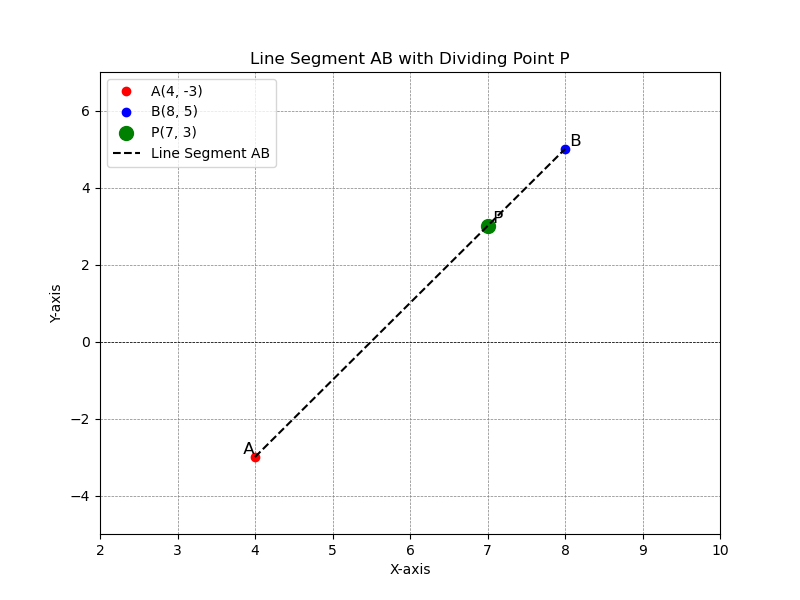
\includegraphics[width=0.6\linewidth]{IMG.png}
   \caption{Stem Plot of y\brak{n}}
     \label{stemplot}
\end{figure}
\begin{table}[h!]
\renewcommand{\thetable}{1}
    \centering
   \begin{tabular}{|c|c|}
    \hline
    {Parameter} & {value}\\ 
    \hline
    $A$ & \brak{4, -3} \\
    \hline 
    $B$ & \brak{8, 5}\\
    \hline
    $P$ & \brak{7, 3}\\
    \hline   
    \end{tabular}
   \def\tablename{Table}
   \caption{Parameters Used}
\end{table}
\end{document}  
